\chapter{Probleme}
\label{cha:Probleme}

\section{Kinect - unnatürliche Farben}
\label{sec:farben}
Die Kamera der Kinect hat eine unnatürliche Farbdarstellung.
Es sind sind starke Unterschiede zwischen Kamerabild und der Wirklichkeit zur erkennen.

\begin{figure}[ht]
	\centering
	\begin{subfigure}{0.45\textwidth}
		\centering
		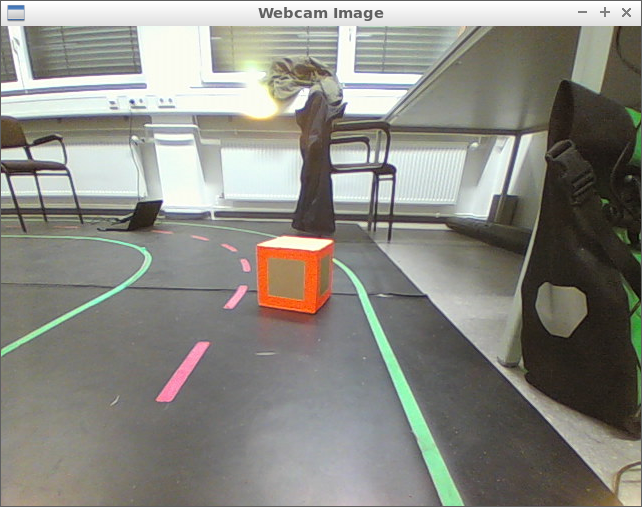
\includegraphics[width=0.9\textwidth]{images/Webcam_RAW.png}
		\caption{Webcam Original}
	\end{subfigure}
	\begin{subfigure}{0.45\textwidth}
		\centering
		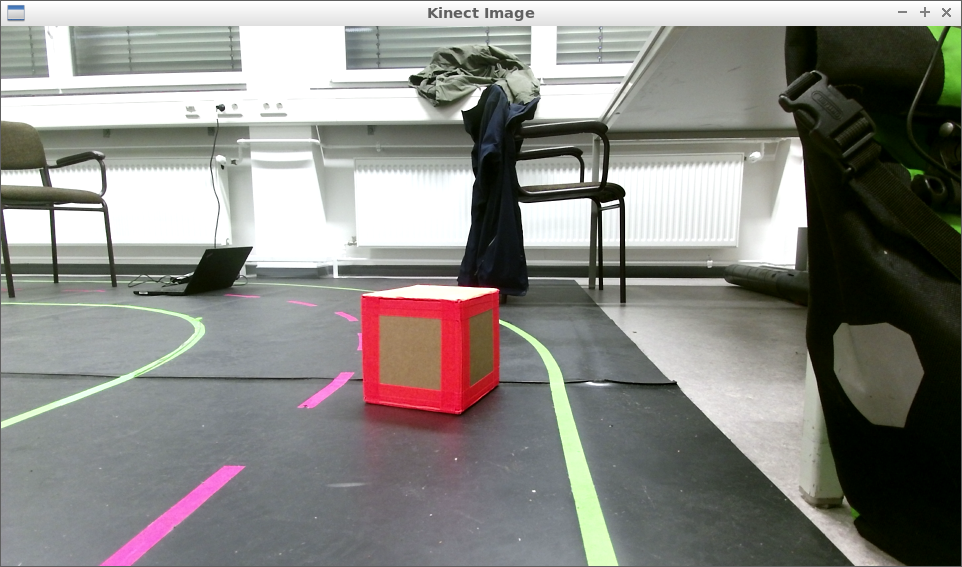
\includegraphics[width=0.9\textwidth]{images/Kinect_qHD_RAW.png}
		\caption{Kinect Original}
	\end{subfigure}
	\caption{Farbdarstellung von Webcam und Kinect}
\end{figure}

Die Farben der Kinect sind übersaturiert und haben teilweise nicht einmal den richtigen Farbton.

\section{Kinect - kleines Sichtfeld}
\label{sec:sichtfeld}
Das Sichtfeld der Kinect Kamera fällt relativ klein aus.
Das hat auch damit zu tun, dass die Kinect in einem Winkel auf dem Fahrzeug angebracht ist, mit dem das Sichtfeld erst circa 30cm vom Fahrzeug entfernt beginnt.
Dadurch kann der Abstand des Fahrzeuges zur Fahrbahnbegrenzung zum aktuellen Zeitpunkt nicht ohne weiteres bestimmt werden. 
Zudem ist die Kamera in der Kinect am rechten Rand platziert.
Dadurch ist die linke Fahrbahnbegrenzung häufig nicht im Sichtfeld.
Dieser Effekt wird noch durch die Transformation zum Bird-Eye View verstärkt.

\begin{figure}[ht]
	\centering
	\begin{subfigure}{0.45\textwidth}
		\centering
		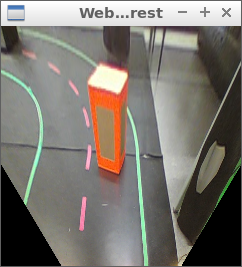
\includegraphics[width=0.9\textwidth]{images/Webcam_BirdEye_ROI.png}
		\caption{Webcam Bird-Eye View und Bildausschnitt}
	\end{subfigure}
	\begin{subfigure}{0.45\textwidth}
		\centering
		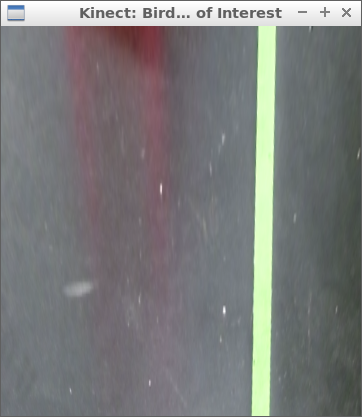
\includegraphics[width=0.9\textwidth]{images/Kinect_BirdEye_ROI.png}
		\caption{Kinect Bird-Eye View und Bildausschnitt}
	\end{subfigure}
	\caption{Sichtfeld von Webcam und Kinect}
\end{figure}

Um eine robuste Fahrbahnerkennung zu implemetieren, sind ordentliche Ausgangsdaten von großer Wichtigkeit.
In unserem Fall benötigen wir eine natürliche Farbdarstellung, ein ausreichend großes Sichtfeld das möglichst nah am Fahrzeug beginnt und eine flüssige Bildrate. 
Alle diese Anforderungen werden von der Webcam erfüllt.
Die Webcam kann zudem sehr flexibel auf dem Fahrzeug angebracht werden.
\\
Die Halterung der Webcam verursacht allerdings ein weiteres Problem.
Die Webcam sakt durch Vibrationen die beim Fahren entstehen nach einiger Zeit etwas ab.
Das heißt die Webcam zeigt mehr in Richtung Boden.
Das hat merkliche Auswirkungen auf die Transformation zum Bird-Eye View.
Wenn der Bird-Eye View nicht mehr korrekt berechnet wird, funktioniert die Erkennung der Fahrsituation nicht mehr so gut.
Genauer wird nicht mehr erkannt, wann sich das Fahrzeug auf einer Geraden befindet.
Da die Regelung abhängig von der Fahrsituation ist, kann das Fahrverhalten schlechter werden.

\section{Webcam verändert Belichtung zur Laufzeit}
\label{sec:belichtung}
Die Webcam passt ihre Belichtung an die aktuellen Lichtverhältnisse zur Laufzeit an.
Das führt leider dazu, dass selbst kleine Veränderungen der Lichtverhältnisse die Belichtung ändern, wie zum Beispiel Lichtspiegelungen auf dem Boden.
Wenn sich die Belichtung ändert, ändern sich auch schlagartig die Farbwerte.
Um keine komplizierte Anpassung der Filterparameter während der Laufzeit vornehmen zu müssen, muss die Belichtung konstant gehalten werden.
Das ist bei dieser Webcam nicht in Software machbar.
Wir haben einen pragmatischen Ansatz gewählt um dieses Problem zu lösen.
Wir blenden die Webcam mit einer LED Leiste.
Die LED Leiste wird über das 12V Boardnetz gespeißt.
Damit nimmt die Webcam die Umgebung immer sehr hell wahr.
Leichte Veränderungen der tatsächlichen Lichtverhältnisse werden durch das Blenden einfach herausgefiltert. 
Das Ergebnis ist eine konstante Belichtung und somit auch konstante Farbwerte.

\section{Fahrwerk}
\label{sec:fahrwerk}
Die Räder kollidieren bei zu hohem Lenkwinkel mit dem Gehäuse.
Deswegen begrenzen wir den maximalen Lenkwinkel auf einen ausgemessenen Wert.
\\
Die Lenkmechanik des Fahrzeugs ist aus Plastik und nicht sonderlich genau gefertigt.
Das hat zur Folge, dass die Lenkung ein merkliches Spiel hat. 
Für uns bedeutet das, dass kleine Veränderungen am Lenkwinkel keine realen Auswirken haben. 
Außerdem liegt relativ viel Last auf der Vorderachse, weil der Laptop Akku und die Kinect vorne im Fahrzeug platziert sind.
Dadurch wird die Lenkmechanik noch zusätzlich belastet.
Bei höheren Geschwindigkeiten sollte sich dieser Effekt allerdings abschwächen. 
Durch diese Effekte können wir uns nicht darauf verlassen, dass nach dem Einstellen eines Lenkwinkels, dieser auch tatsächlich anliegt.
In der Praxis fahren wir allerdings immer mindestens so schnell, dass dieser Effekt keine allzu großen Auswirkungen hat.
\\
Ein weiteres Problem besteht darin, dass der Lenkwert der an die UC\_Bridge gesendet wird, sich nicht linear in einen Lenkwinkel umrechnen lässt.
Die Beziehung zwischen Lenkwert und Lenkwinkel auszumessen gestaltet sich schwierig.
Da diese Beziehung stark von der Geschwindigkeit und der Last auf die Lenkmechanik abhängt.
Wenn der tatsächliche Lenkwinkel durch passende Sensoren regelmäßig gemessen werden würde, könnte man eine Regelung für den Lenkwinkel konzipieren.
Wir haben uns um dieses Problem nicht weiter gekümmert und haben uns stattdessen darauf konzentriert eine möglichst robuste Regelung zur Fahrspurhaltung zu implementieren.
Um die Lenkmechanik nicht unnötig zu belasten haben wir eine möglichst ruhige Regelung vorgenommen.




